
\newcommand{\printfigTypes}{
    \begin{figure}
        \begin{subfigure}{.5\textwidth}
            \centering
            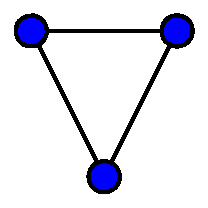
\includegraphics[width=.8\linewidth]{assets/images/Undirected.svg.pdf}
            \caption{1a}
            \label{fig:sfig1}
        \end{subfigure}%
        \begin{subfigure}{.5\textwidth}
            \centering
            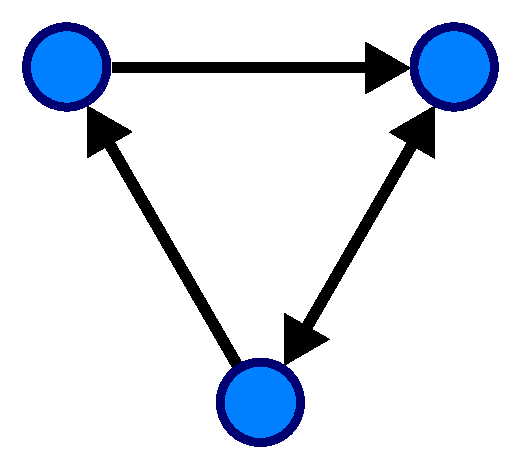
\includegraphics[width=.8\linewidth]{assets/images/Directed.svg.pdf}
            \caption{1b}
            \label{fig:sfig2}
        \end{subfigure}
        \begin{subfigure}{.5\textwidth}
            \centering
            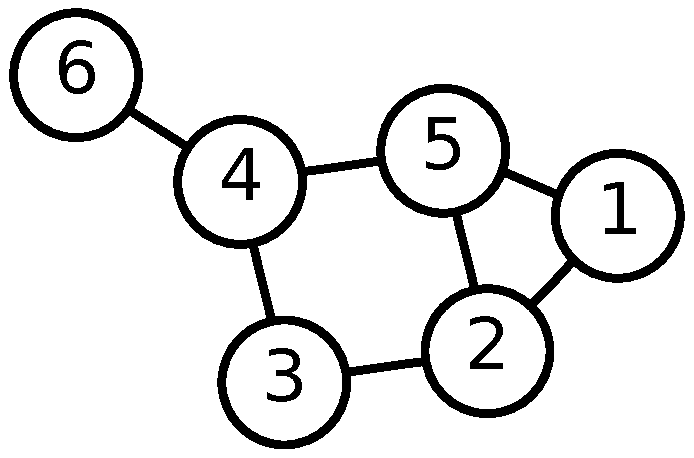
\includegraphics[width=.8\linewidth]{assets/images/6n-graf.svg.pdf}
            \caption{1a}
            \label{fig:sfig1}
        \end{subfigure}%
        \begin{subfigure}{.5\textwidth}
            \centering
            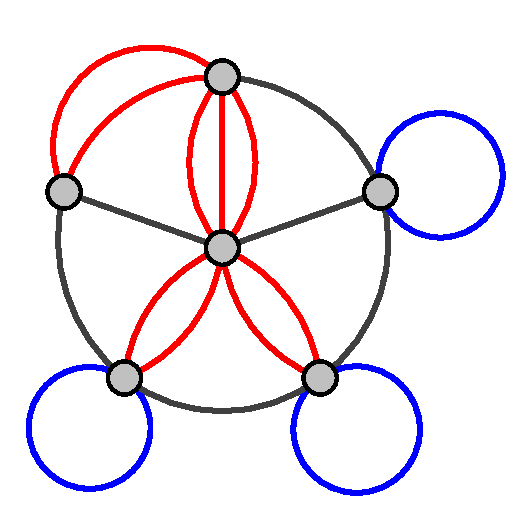
\includegraphics[width=.8\linewidth]{assets/images/Multi-pseudograph.svg.pdf}
            \caption{1b}
            \label{fig:sfig2}
        \end{subfigure}
        \begin{subfigure}{.5\textwidth}
            \centering
            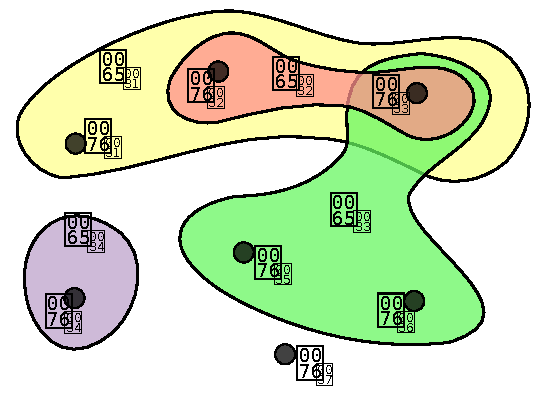
\includegraphics[width=.8\linewidth]{assets/images/Hypergraph-wikipedia.svg.pdf}
            \caption{1a}
            \label{fig:sfig1}
        \end{subfigure}%
        \begin{subfigure}{.5\textwidth}
            \centering
            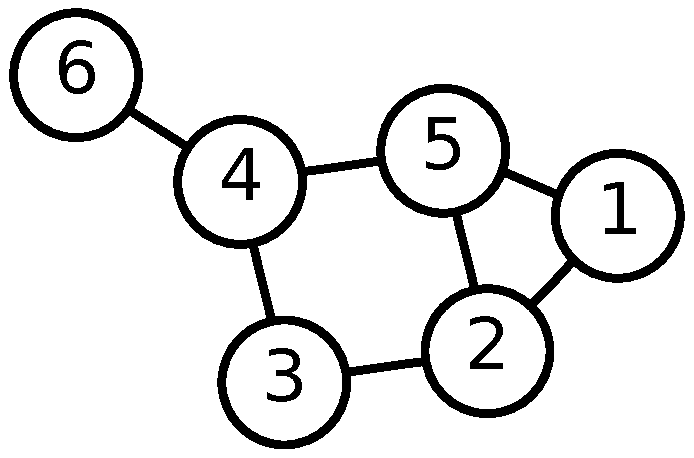
\includegraphics[width=.8\linewidth]{assets/images/6n-graf.svg.pdf}
            \caption{1b}
            \label{fig:sfig2}
        \end{subfigure}
        \caption{plots of....}
        \label{fig:fig}
    \end{figure}
}